% vim: textwidth=75 rnu ts=2 sw=2 et

% superscriptaddress - don't group by affiliation
% nofootinbib - footnote doesn't go in bibliography
% endfloats - put floats together at the end
% endfloats* - every float will be on its own page
\documentclass[superscriptaddress,nofootinbib,twocolumn]{revtex4-1}

\usepackage{amsmath}
\usepackage{amssymb}

\usepackage{hyperref}              % revtex will link biblio
\usepackage{cleveref}  % Better figures/equations references
                                   % hyperref must come before cleveref

\usepackage{color}      			     % Colored text
\usepackage{soul}                  % Hyphenation, strikethrough
\usepackage{graphicx}              % Figures
\usepackage{siunitx}				       % SI Units

\hyphenation{MSMBuilder}

\begin{document}
\title{MSMBuilder: Statistical Models for Biomolecular Dynamics}
\date{\today}

\author{Matthew P. Harrigan}
\affiliation{Department of Chemistry, Stanford University, Stanford, CA 94305}

\author{Mohammad M. Sultan}
\affiliation{Department of Chemistry, Stanford University, Stanford, CA 94305}

\author{Carlos X. Hern\'andez}
\affiliation{Program in Biophysics, Stanford University, Stanford, CA 94305}

\author{Brooke E. Husic}
\affiliation{Department of Chemistry, Stanford University, Stanford, CA 94305}

\author{Peter Eastman}
\affiliation{Department of Chemistry, Stanford University, Stanford, CA 94305}

\author{Christian R. Schwantes}
\affiliation{Department of Chemistry, Stanford University, Stanford, CA 94305}

\author{Kyle A. Beauchamp}
\altaffiliation[Current address: ]{Counsyl, 180 Kimball Way, South San Francisco, CA 94080}
\affiliation{Memorial Sloan Kettering Cancer Center, New York, NY 10065}

\author{Robert T. McGibbon}
\email[Co-corresponding author: ]{Robert.McGibbon@DEShawResearch.com}
\altaffiliation[Current address: ]{D. E. Shaw Research, 120 W. 45th St., 34th Fl. New York, NY 10036}
\affiliation{Department of Chemistry, Stanford University, Stanford, CA 94305}

\author{Vijay S. Pande}
\email[Co-corresponding author: ]{pande@stanford.edu}
\affiliation{Department of Chemistry, Stanford University, Stanford, CA 94305}
\affiliation{Department of Computer Science, Stanford University, Stanford, CA 94305}
\affiliation{Department of Structural Biology, Stanford University, Stanford, CA 94305}
\affiliation{Program in Biophysics, Stanford University, Stanford, CA 94305}


\begin{abstract}

MSMBuilder is a software package for building statistical models of
high-dimensional time-series data. It is designed with a particular focus
on the analysis of atomistic simulations of biomolecular dynamics such as
protein folding and conformational change.  MSMBuilder is named for its
ability to construct Markov State Models (MSMs), a class of models that has
gained favor among computational biophysicists.  In addition to traditional
and cutting-edge flavors of MSMs, the package includes complementary
algorithms for understanding time-series data such as hidden Markov models
(HMMs) and time-structure based independent component analysis (tICA).
MSMBuilder boasts an easy to use command-line interface, as well as clear
and consistent abstractions through its Python API (application programming
interface).  MSMBuilder is developed with careful consideration for
compatibility with the broader machine-learning community by following the
design of \texttt{scikit-learn}.  The package is used primarily by
practitioners of molecular dynamics but is just as applicable to other
computational or experimental time-series measurements.
\url{http://msmbuilder.org}

\end{abstract}

\maketitle


\section{Introduction}
\label{sec:intro}
Molecular dynamics (MD) is a powerful probe into atomistic dynamics. Recent
advances in technology (specialized hardware \cite{2008-anton} or commodity
GPUs \cite{2009-friedrichs-gpu}) and strategies (massively distributed
architectures \cite{2000-fah, 2010-gpugrid, 2014-kohlhoff-exacycle}) enable
simulations to reach larger size and longer timescales. Increasing
quantities of raw data require novel and sophisticated analysis techniques
\cite{2014-msm-perspective}. Markov state models (MSMs) have gained favor
for drawing interpretable conclusions from time-series data
\cite{2010-everything-msm-afraid-ask, 2014-msm-perspective,
2014-chodera-msm, 2014-msm-book}. Briefly, MSMs model dynamic systems using
a set of discrete states and pairwise transition rates. From these models,
the researcher can compute observables of interest and make predictions.
These models are statistically rigorous and easy to
interpret. Furthermore, MSMs are able to stitch together many
independent simulation runs, allowing researchers to fully exploit
distributed computing.

The idea of describing a system by its states and rates is natural for
chemists and biologists, but the estimation of states and rates from finite
data (perhaps molecular dynamics) is not obvious. From the introduction of
MSMs to the biophysics community, algorithmic improvements for constructing
MSMs and computing observables have been the focus of intense study. The
practical implementation of these algorithms has spawned several historical
packages for MSM construction \cite{2009-msmbuilder1, 2011-msmbuilder2,
2012-jemma}. Each of these packages was tied strongly to the best
practices in MSM construction of the time. Due to the fast-moving research
around MSMs, software re-writes were common \cite{2015-pyemma, 2016-htmd}.

We introduce MSMBuilder~3, a community-driven, open source software package
for constructing MSMs. MSMBuilder offers a curated selection of MSM
construction algorithms based on modern advances in the field. MSMBuilder
is implemented in the Python programming language with performance-critical
components written in C. It exposes an extensible API modeled after that of
\texttt{scikit-learn}. The modular design ensures MSMBuilder~3 is adaptable
to future improvements in MSM construction. The package can be invoked
directly from Python or via the command line.

Through two instructive examples, we showcase the capabilities
of MSMBuilder. In the first, we use MSMBuilder to analyze a biological
system of interest from a dataset composed of more than 20,000
trajectories. This example builds a single MSM using methods
unavailable in previous tools.
Due to rapid advances in MSM methods,
a variety of modeling choices are now available to researchers. 
In the second example, we demonstrate how MSMBuilder's
implementation of scoring functionals
can be used to choose among these methods.

% vim: tw=75


\section{Instructive Examples}
\subsection{Constructing an MSM}
\label{sec:example-src}
\begin{figure}[htbp]
\centering
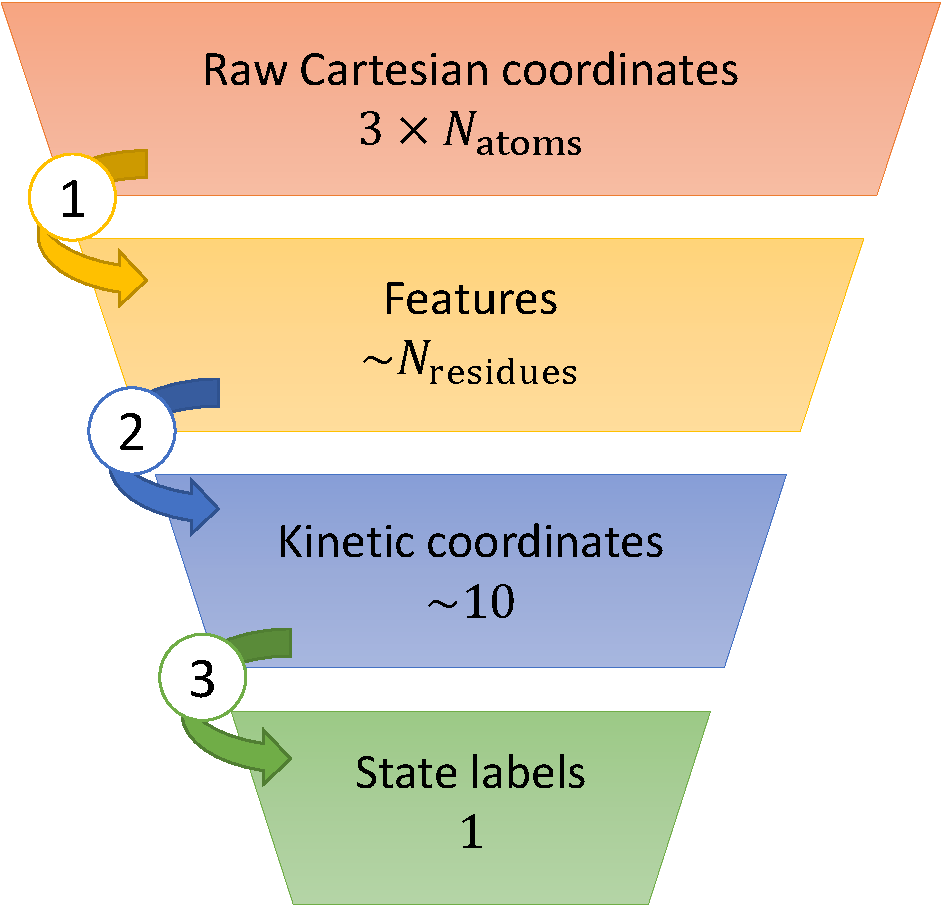
\includegraphics[width=0.9\linewidth]{1-src/dimreduce}
\caption{\textbf{Data transformations and their dimensionality.}
    Markov state models (MSMs) partition dynamical data into a set of
    states and estimate rates between them. A typical pipeline for state
    definition consists of a series of transformations (indexed by circled numbers)
    between representations of the data. Each step projects a higher
    dimensional representation onto a lower dimensional representation. The
    approximate dimension of each representation is reported below the
    representation name.
    Although not traditionally thought of as a 
    dimensionality reduction, clustering (step 3) 
    reduces each frame to a single integer cluster label.
}
\label{fig:dimreduce}
\end{figure}

\begin{figure}[htbp]
\centering
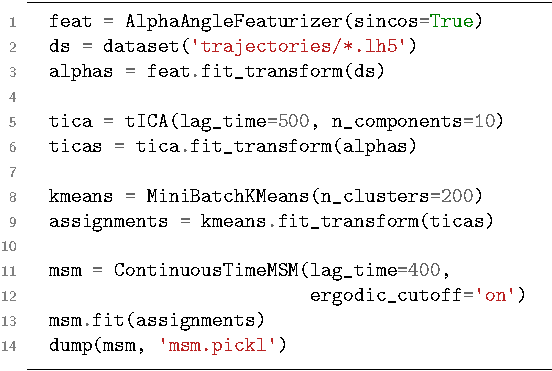
\includegraphics[width=\linewidth]{1-src/code}
\caption{\textbf{Sample MSM code.}
    MSMBuilder balances a powerful API (application programming interface) with ease of use.
    A sample workflow
    is shown here using the Python API. Following the successful model of
    the broadly-applicable \texttt{scikit-learn} package, each modelling step is
    represented by an estimator object which operates on the data. Here, the
    \texttt{AlphaAngleFeaturizer} transforms raw coordinates into
    $\alpha$ angles. The output of this transformation is fed into the
    \texttt{tICA} dimensionality reduction, \texttt{MiniBatchKMeans}
    clustering algorithm, and finally into the \texttt{ContinuousTimeMSM}
    model. MSMBuilder provides a litany of utility functions for dealing
    with large molecular dynamics datasets for I/O. While this example
    shows the Python API, MSMBuilder is fully functional from the command
    line with an intuitive 1-to-1 correspondence between Python estimator
    objects and command-line commands.
}
\label{fig:src-code}
\end{figure}

\begin{figure}[htbp]
\centering
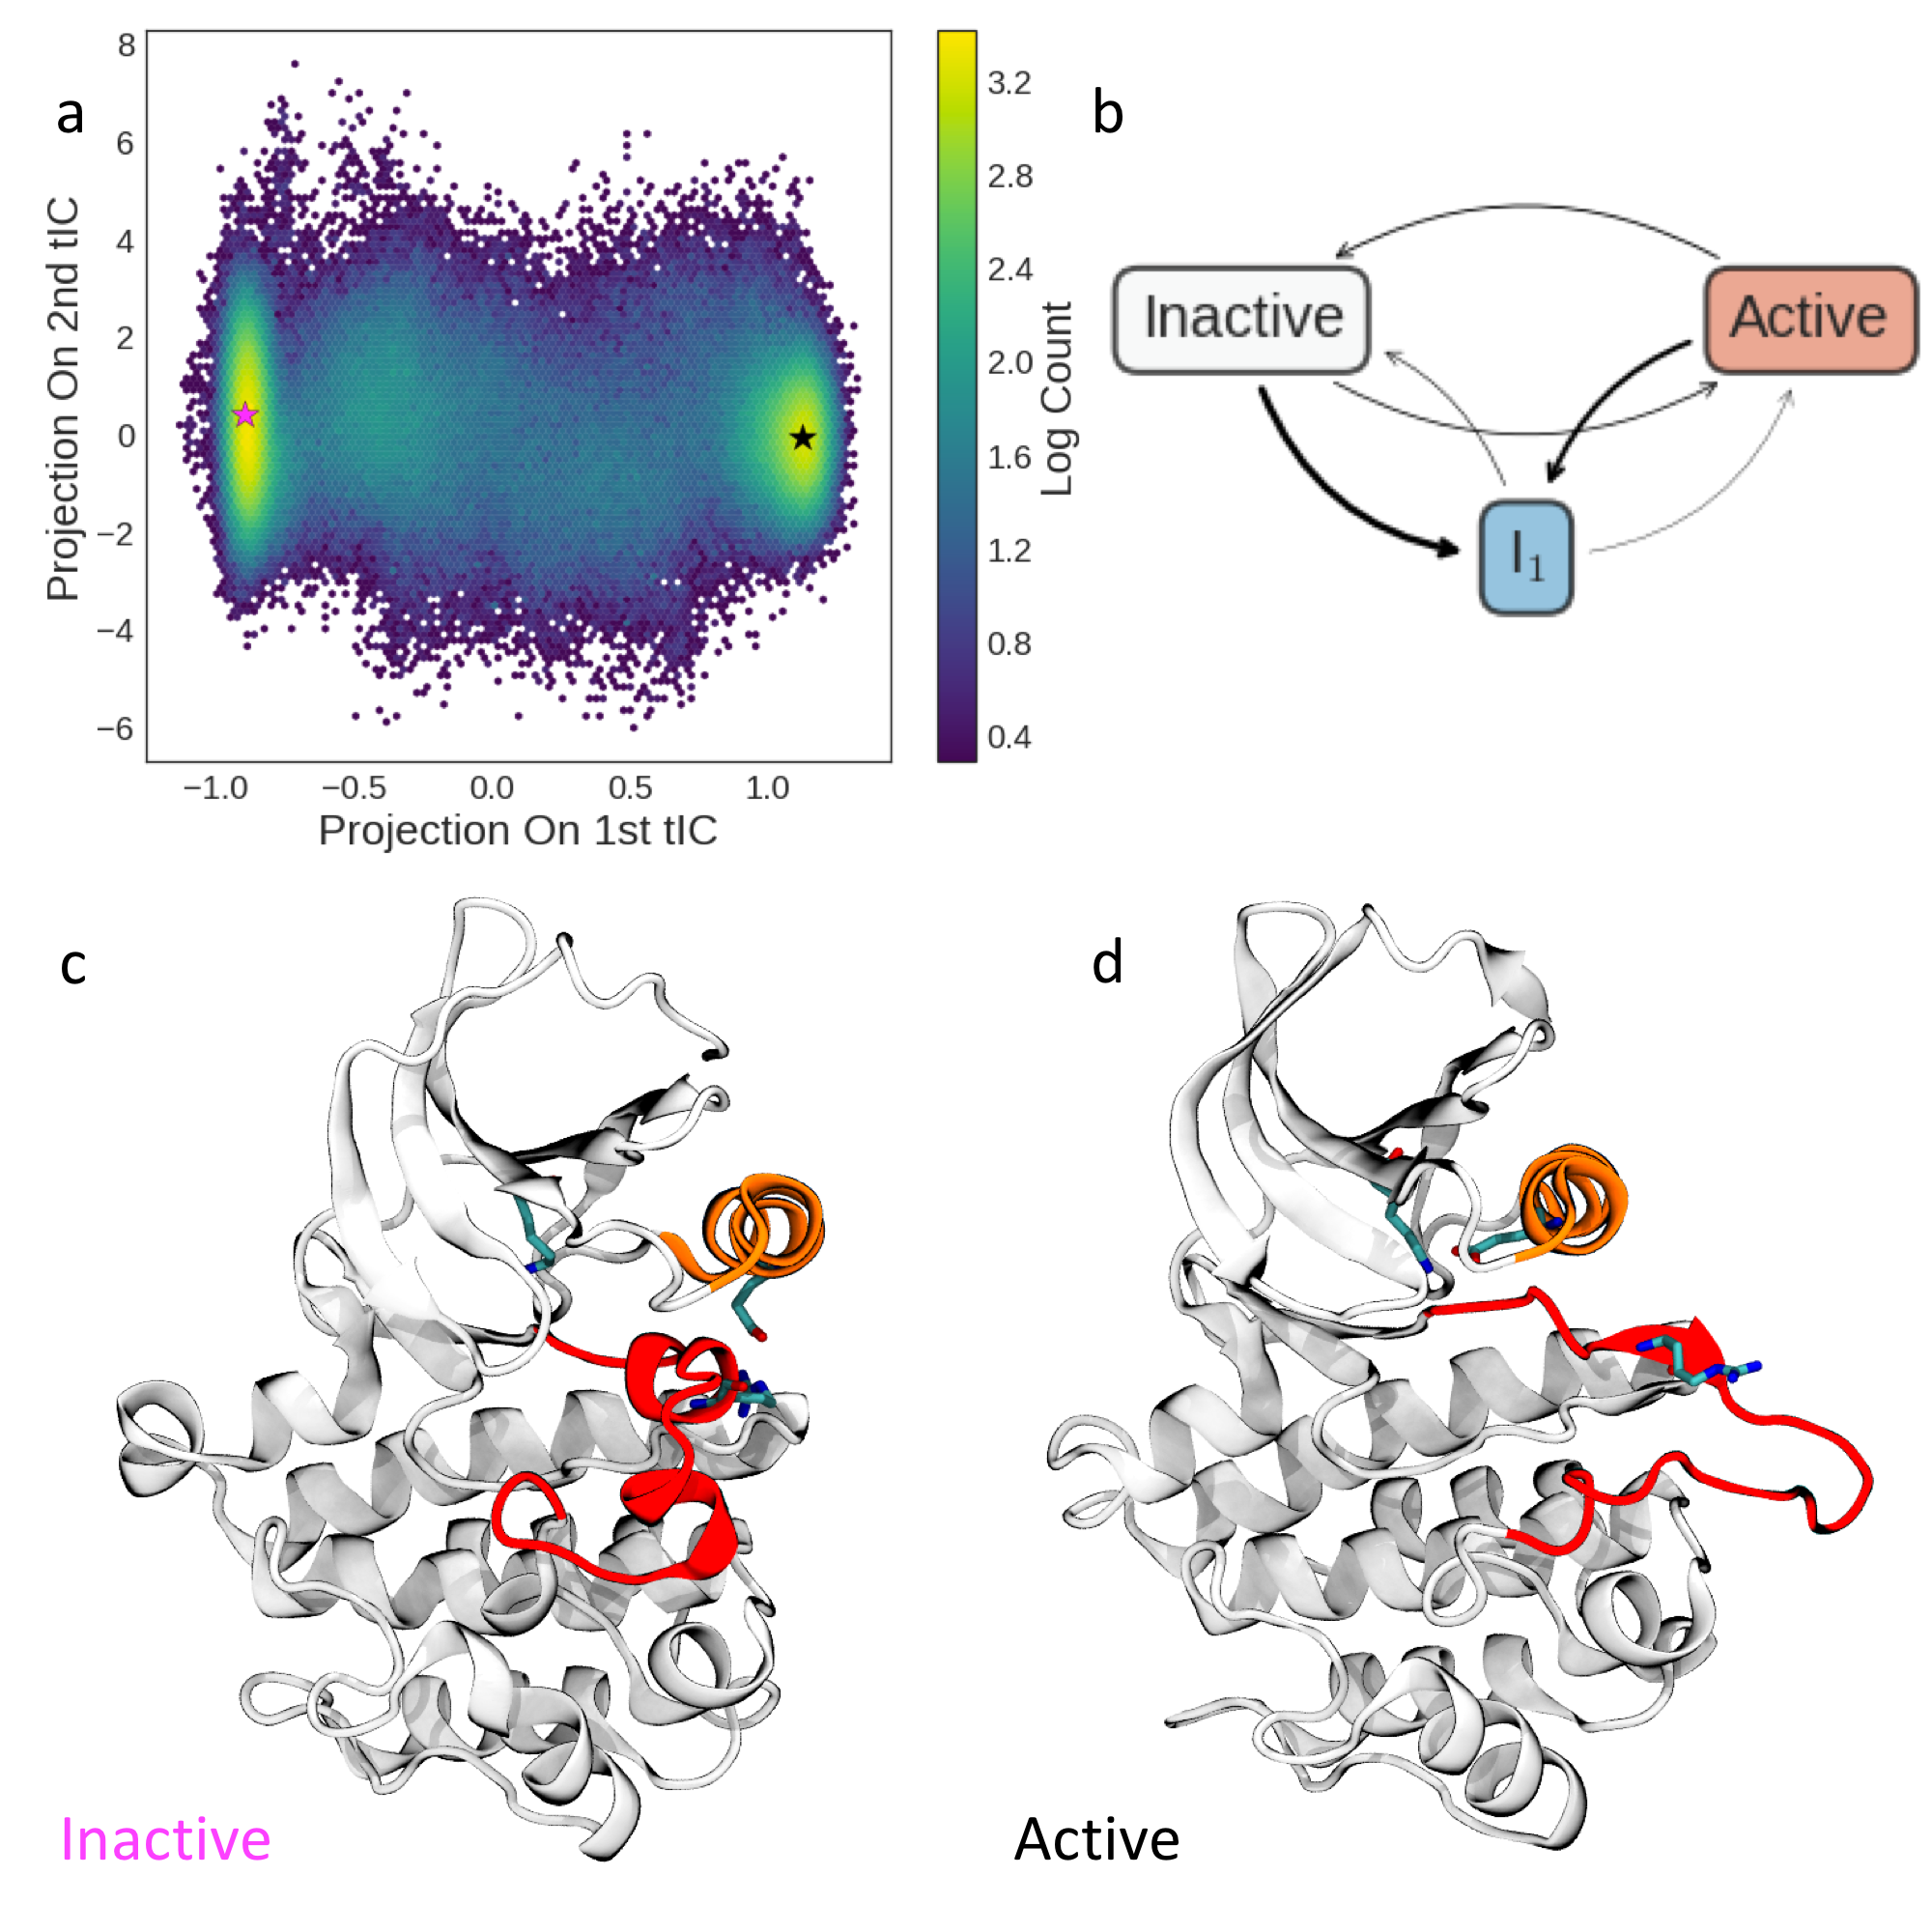
\includegraphics[width=\linewidth]{1-src/plot}
\caption{\textbf{c-Src kinase MSM.}
    MSMBuilder constructs interpretable models from large datasets.  This
    figure shows a 2D-histogram for the Src kinase from tICA-MSM analysis
    projected onto the dominant modes of a tICA model (a).  A simple
    macrostate model of the dynamics shows the presence of an intermediate
    state I$_1$ connecting the inactive and active states (b). The arrow
    thickness corresponds to the rate of transitions. The model
    indicates that the active state (red) is the most stable state followed
    by the inactive and intermediate states (gray and blue, resp.).
    The analysis discovers a coordinate (the first tIC) between the known
    active and inactive conformations. Representative structures
    are selected from MSM states and show the conformational differences
    between the two basins. The unfolding of the activation loop (red
    helix) forms a catalytically active Src capable of initiating and
    regulating downstream signaling pathways (c and d). 
}
\label{fig:src}
\end{figure}

MSMBuilder allows rapid analysis of large molecular dynamics datasets. In
this example, we construct an MSM of a kinase molecule.  Kinases are
critical enzymes that control cellular pathways. Malfunctions of kinases
have been linked to many different cancers
\cite{Taylor_TrendsBiochemSci11}.  Here, we use MSMBuilder to study the
c-Src kinase, a regulator of cellular growth \cite{Shukla_NatCommun14}, and
demonstrate that the resulting MSM can capture activation dynamics.
Understanding the activation process reveals atomistic, kinetic,
and thermodynamic insights into the protein's conformational
heterogeneity, which can help design better therapeutics.

Broadly, the procedure for constructing an MSM is to define a set of states
and then estimate transition rates among those states.  Before beginning
model construction, researchers must obtain time-series data they wish to
model.  Usually, this is the output of a molecular dynamics engine
(MSMBuilder supports nearly every MD trajectory file format \cite{2015-mdtraj}), 
but it
could also be experimental time-series measurements. For this example, we
use a previously-generated MD dataset of the c-Src kinase, publicly
available from the Stanford Digital Repository (SDR) \footnote{Available here:
https://goo.gl/LLchMT.  For simulation details, see
\citet{Shukla_NatCommun14}.}. 

The first step of model construction is to transform the raw Cartesian
coordinates into vector features that respect the physics of the system,
namely translational and rotational invariance (\cref{fig:dimreduce}, step
1).  Here, we project our trajectory frames onto the dihedral angles
created by each set of four consecutive alpha carbons ($\alpha$ angles)
\cite{Flocco_ProteinSci95}.  This reduces the dimensionality of the data
from 12,693 Cartesian coordinates to 518 features.  The appropriate
featurization depends on the particular system under study (see \cref{sec:example-gmrq}). MSMBuilder
offers a collection of featurization strategies with a unified interface.
Popular features include backbone and side chain dihedrals (through the
\texttt{DihedralFeaturizer} class), heavy atom or  C$_\alpha$ contact
distances (\texttt{ContactFeaturizer}), distance of reciprocal inter-atomic
distances (\texttt{DRIDFeaturizer}) \cite{2012-drid}, and root mean squared
deviation to a set of structures (\texttt{RMSDFeaturizer}). There are
additional utilities for concatenation of multiple choices of features and
feature scaling.
% Note: ariana thinks that feature scaling needs more explanation
% I can't think of a way to describe it without messing up the flow of
% this section. Plus there is a wikipedia article named "feature scaling",
% so I don't think it's too unique a term.

The second step in MSM construction projects structural features onto
kinetically-motivated coordinates (\cref{fig:dimreduce}, step 2).  Through
our ``state" definition, we assert that conformations within a state
interconvert rapidly. By moving from a structural representation of our
data to a kinetic one, we can capture the essential dynamics with fewer
dimensions (typically of order 10).  To achieve this, we use
time-structure based independent
component analysis (tICA) to learn a small number of kinetic coordinates
onto which we projected our features from the previous step
\cite{2013-schwantes-tica, 2013-noe-tica}. This reduced the dimensionality
of our kinase data from 518 dihedrals to 5 kinetic coordinates.  MSMBuilder
includes support for more advanced kinetic coordinate determination
(\texttt{SparseTICA} \cite{2016-sparsetica}) as well as general manifold
learning algorithms like principal components analysis (\texttt{PCA}),
\texttt{SparsePCA}, or \texttt{MiniBatchSparsePCA}. Prior to 2013, this
step was not available for model construction. Accordingly, software
available at the time could not easily be extended to accomodate tICA
intermediate processing. The design of MSMBuilder~3 permits arbitrary
addition, subtraction, and re-ordering of data transformation steps.

Next, we define the states of our MSM by grouping conformations which
interconvert rapidly (\cref{fig:dimreduce}, step 3). For the c-Src kinase,
we employ the \texttt{MiniBatchKMeans} \cite{2010-minibatch-kmeans}
clustering algorithm to parition our data into 200 microstates. We note
that our data has been reduced from 5 kinetic
coordinates to one integer cluster label per frame. 
The prior transformation into kinetic
coordinates permits using off-the-shelf clustering algorithms. Accordingly,
MSMBuilder supports K-Means like clustering algorithms (\texttt{KCenters},
\texttt{KMedoids}, and  \texttt{MiniBatchKMedoids}), and hierarchical clustering.

With our states defined, we proceed to estimate the rates among them. As
the final model construction step, we learn a continuous-time MSM
\cite{2015-ratematrix} from our labeled trajectories. We have chosen to use
a continuous-time MSM to directly estimate transition rates; we could have
alternatively built a traditional MSM (to estimate transition
probabilities) or a hidden Markov model (HMM). We direct interested readers
to a more thorough application of HMM modelling to the c-Src dataset
\cite{2014-hmm}. The relevant Python code for constructing this MSM is
shown in \cref{fig:src-code}. Complete, executable code is available in the
SI as an IPython \cite{2007-ipython} notebook.

To draw interpretable conclusions from our data via Markov modelling, we
query the model.  For c-Src, we use MSMBuilder to relate model behavior to
biological function.  We present a log-scaled 2D histogram
(\cref{fig:src}a) of the trajectories projected onto the two dominant slow
processes, or ``tICs'', from our tICA model. We then sample the centroids
of states (shown as pink and black stars) in low free energy regions to
visualize representative configurations in three dimensions \cite{1996-vmd}
(\cref{fig:src}c and d). The dominant tIC (x-axis) highly correlates with
the activation of the kinase. Kinase activation requires the unfolding of
the activation loop (red) and an inward swing of the catalytic helix
(C-helix). The inward rotation of the helix coincides with the switching of
hydrogen bonding pair from Glu-Arg  to Glu-Lys (licorice). We investigate
the dynamics between the active, inactive, and intermediate macrostates by
applying Robust Perron Clustering Analysis (PCCA+) to our MSM. PCCA+ is a
spectral clustering method, which lumps MSM states into an arbitrary number
of metastable macrostates, facilitating qualitative analysis of rates and
populations among biologically-relevant macrostates \cite{2005-pcca}. The
rates among three macrostates are shown by the thickness of arrows in
\cref{fig:src}b. Further options of querying the model (not shown here but
available in MSMBuilder) include computation of relaxation timescales,
transition path theory analysis \cite{Metzner_MMS09, Berezhkovskii_JCP09,
Noe_PNAS09}, and generation of synthetic trajectories for visual
inspection.

The assortment of modeling options such as the choice of featurizer, the
use of dimensionality reduction, and the selection of the clustering
algorithm, along with any associated internal parameter choices, presents
the modeler with a motley of modeling decisions and tunable parameters.
In the next
section, we show how a scoring metric for MSMs can provide the modeler with
a unbiased protocol for determining which parameters are suitable given a
set of MD trajectories.

% vim: tw=75


\subsection{Selecting Hyperparameters}
\label{sec:example-gmrq}
\begin{figure}[htbp]
\centering
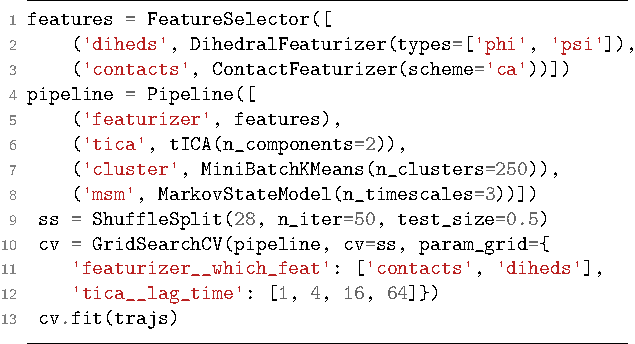
\includegraphics[width=\linewidth]{2-gmrq/code}
\caption{\textbf{Sample GMRQ code.}
    MSMBuilder seamlessly interoperates with the broader Python ecosystem.
    In this code sample, we use \texttt{scikit-learn} for
    algorithm-agnostic data processing and MSMBuilder for
    biophyics-oriented time-series algorithms with the goal of selecting
    model hyperparameters.  Our analysis pipeline is similar to that of
    \cref{sec:example-src} but with a choice of features (between dihedrals
    and contact distances) and tica lag times (among 1, 4, 16, and 64
    steps).  The \texttt{ShuffleSplit} cross-validation scheme runs 50
    iterations of equal partitioning of the 28 trajectories between train and test
    sets, and we perform a full grid-search over parameter choices.  We can
    plot the distribution of scores vs. parameters as in
    \cref{fig:gmrq}.
}
\label{fig:gmrq_code}
\end{figure}

\begin{figure}[htbp]
\centering
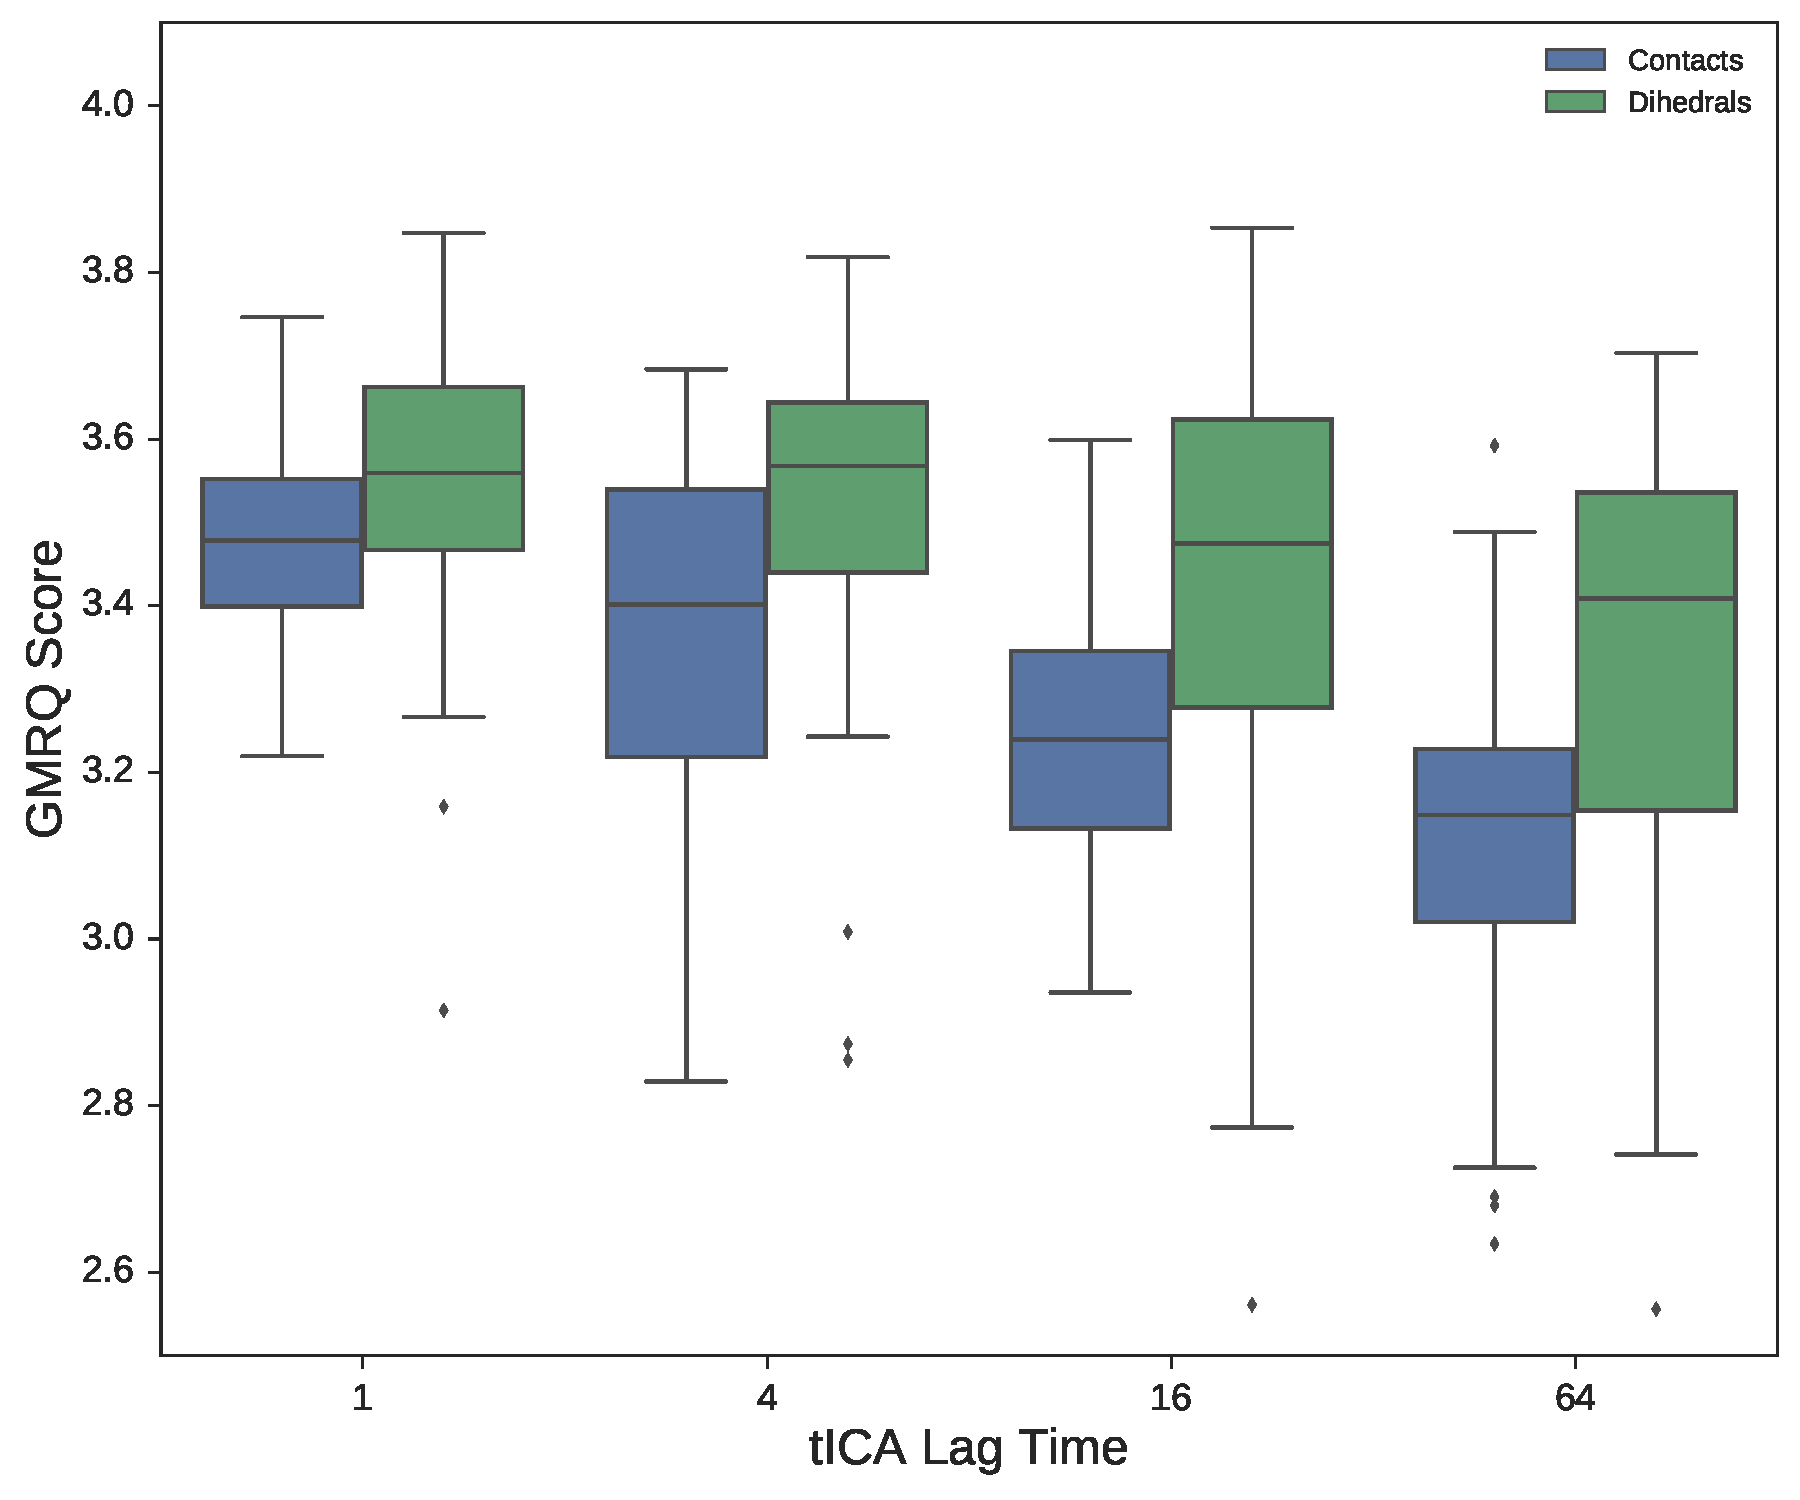
\includegraphics[width=\linewidth]{2-gmrq/plot}
\caption{\textbf{GMRQ parameter selection.}
    MSMBuilder offers robust machinery for selecting hyperparameters that
    cannot \emph{a priori} be learned from the data. Here, we perform
    shuffle-split cross validation over choices of featurization and tICA
    lag time. Historically, these parameters were chosen heuristically.
    With the advent of the GMRQ score and its implementation in MSMBuidler,
    we can choose these parameters in a statistically rigorous way. Here,
    we plot the distribution of scores for each set of of model parameters.
    Note that a higher score is generally an indication of a more predictive
    model. In this example, we find that featurization with dihedral angles
    at a lag time of 4 steps has highest median score and recommend this
    hyperparameter set to be chosen for the final model.
}
\label{fig:gmrq}
\end{figure}

Historically, the heuristic choice of hyperparameters---choices of
protocol---rendered MSM construction as much of an art as a science. It is
clear from \cref{sec:example-src} that there is an abundance of algorithms
available in MSMBuilder. In this instructive example, we use a
scoring functional to select the best models.

\citet{2014-noe-variational} introduced a variational principle that
formalized the definition of a ``good" MSM. In keeping with inspiration
from the broader machine learning community, MSMBuilder extends this
formalism in the context of cross-validation through the work of
\citet{2015-gmrq}. The resulting generalized matrix Rayleigh
quotient (GMRQ) score offers an objective way to pick the best model (i.e. the
appropriate modeling choices) from the given data. Briefly, the GMRQ measures
the ability of a model to capture the slowest dynamics of a system. The
variational principle states that approximating the full phase space
by discrete states  will always yield dynamics that are too fast.
The GMRQ score is a summation of the leading eigenvalues of the model
and therefore provides a measure of ``slow-ness".
A higher score means the model is closer to the variational bound, and
therefore should be prefered over lower scoring models.

In this example, we use the GMRQ score under cross-validation to evaluate
the relative merit of enumerated hyperparameter values when constructing a
model for the Fs peptide \cite{2014-fs-peptide}. The relevant code in
\cref{fig:gmrq_code} sets up a choice between two structural features
(dihedral angles or contact distances) and a choice among tICA lag times.
We perform shuffle-split cross-validation by randomly assigning the 28
trajectories to either the training set or test set. The MSM is learned on
the training set and scored on the test set. By concealing the training
data during scoring, cross-validation guards against overfitting
(overconfidence in excessively complex models). The trajectories are
re-shuffled and this process is repeated to compute an average score for a
given set of hyperparameters.  The scores for each of the 50
cross-validation splits are plotted in a box plot in \cref{fig:gmrq}.
The dihedral angle featurization with a lag-time of 4 steps gives the best model in this
search space.  A simple grid search as performed in this example can become
intractible as the number of hyperparameters (i.e.~the dimension of the
search space) increases. We direct interested users to Osprey
\cite{2016-osprey}, a tool for hyperparameter optimization with a variety
of search strategies and support for parallel computation.
Osprey interoperates with any \texttt{scikit-learn} estimator
including those in MSMBuilder.

This example leverages the \texttt{Pipeline}, \texttt{ShuffleSplit}, and
\texttt{GridSearchCV} machinery from \texttt{scikit-learn}. Additionally,
MSMBuilder uses this library internally for generic machine learning
algorithms such as clustering or PCA. We note that such general algorithms
do not need to be reinvented and re-programmed by the biophysics community.
By delegating some development effort to this widely-used machine learning
library, we ensure that the development of MSMBuilder is focused on
biophysical algorithms and considerations.
This advantage offers rapid adoption of the latest algorithms which have
demonstrated improved ability to build MSMs (e.g. \cite{2015-gmrq}) and a
larger community for code maintenance and longevity.


% vim: tw=75


\section{Conclusions}
\label{sec:conclusion}
MSMBuilder~3 is a powerful and accessible software package for drawing
interpretable conclusions from time-series data. We used two examples to
demonstrate how MSMBuilder can make sense of a molecular dynamics dataset
consisting of thousands of trajectories in a highly automated and
statistically robust way. In the first example, we construct a ``vanilla''
MSM and show how MSMBuilder enables the construction of
interpretable models that expose the connection between biological function
and structural dynamics.  We highlight the breadth of relevant algorithmic choices for
featurization, normalization, dimensionality reduction, clustering, and MSM
modelling.  In the second instructive example, we acknowledge that the
explosion of choices in parameters and protocol can be overwhelming. We use
the GMRQ score and off-the-shelf cross-validation machinery to do a simple
grid search over tunable parameters to evaluate the relative merit of many
MSMs built on the same MD dataset of a small protein. Since
cross-validation is not a technique unique to biophysics, we leverage the
greater Python machine learning ecosystem for this example.

More broadly, MSMBuilder's power and clarity is derived from its integration
with the machine learning community at large. Our power to focus on
developing methods bespoke to biophysics and time-series analysis comes
from exploiting general-purpose algorithms implemented by respective
experts. The clarity of MSMBuilder's API is due in large part to the
massive amount of effort and skill put into the design of
\texttt{scikit-learn}'s API. As distributed computing and Markov modelling
continue to become more prominent, MSMBuilder offers a sustainable,
extensible, powerful, and easy-to-use set of Python and command-line tools
to help researchers draw meaningful conclusions from their data.

% vim: ts=2 sw=2 et tw=75


\section{Availibility}

MSMBuilder documentation and installation is available at
\url{http://msmbuilder.org}. The source code is available under the
open-source LGPL2.1 license and is accessible at
\url{http://github.com/msmbuilder/msmbuilder}.
The current release at time of writing is version 3.5 \cite{2016-msmbuilder3.5-zenodo}. 
Complete examples can be
found as IPython notebooks in the supporting information and at
\url{http://github.com/msmbuilder/paper}.

\section{Author Contributions}

MPH, MMS, CXH, and BEH wrote the paper.
MPH, MMS, CXH, BEH, PE, CRS, KAB, RTM, and VSP edited the paper.
MPH, MMS, CXH, BEH, PE, CRS, KAB, and RTM wrote the software.
VSP supervised the project.

\section{Acknowledgments}

We extend thanks to all our contributors including
Stephen Liu, Patrick Riley, Steven Kearnes, Joshua Adelman, and Gert Kiss.
We acknowledge funding from NIH grants U19 AI109662 and 2R01GM062868.
MMS acknowledges support from NSF-MCB-0954714.
CXH acknowledges support from NSF GRFP (DGE-114747).
KAB acknowledges support from NIH grant P30CA008747, the Sloan Kettering
Institute, and Starr Foundation grant I8-A8-058.
We acknowledge members of the Chodera, Pande, and No\"{e} labs for helpful
discussions. We thank Ariana Peck for invaluable feedback on this manuscript.

\section{Disclosure}
KAB is currently an employee of Counsyl, Inc.
RTM is currently an employee of D.E. Shaw Research, LLC.
VSP is a consultant of Schrodinger, LLC and a member of its scientific
  advisory board.

\bibliography{msmbuilder.bib,msm.bib,tools.bib}


\end{document}
